\newpage
\section{Ôn tập chương 1}
\def\thoigian{90}%--Thời gian
\de{Đề số 1}{Chương I. Ứng dụng đạo hàm để khảo sát hàm số}

\begin{center}
	\textbf{PHẦN 1 - CÂU TRẮC NGHIỆM BỐN PHƯƠNG ÁN}
\end{center}
\Opensolutionfile{ans}[ans/ans-TN-ONTAPCHUONG-DE1]

\begin{ex}%[2D1N1-2]
	Cho hàm số $y=f(x)$ có bảng biến thiên như hình bên dưới. Hàm số $y=f(x)$ nghịch biến trên khoảng nào sau đây?
	\begin{center}
		
\begin{tikzpicture}
			\tkzTabInit[nocadre=false,lgt=1.2,espcl=2.5,deltacl=0.6]
			{$x$ /1,$y'$ /0.6,$y$ /2}
			{$-\infty$,$-\dfrac{1}{2}$,$0$,$\dfrac{1}{2}$,$+\infty$}
			\tkzTabLine{,+,$0$,-,$0$,+,$0$,-,}
			\tkzTabVar{-/$-\infty$, +/$-\dfrac{55}{8}$,-/$-7$,+/$-\dfrac{55}{8}$,-/$-\infty$}
		\end{tikzpicture}
	\end{center}
	\choice
	{\True $\left(-\dfrac{1}{2};0\right)$ và $\left(\dfrac{1}{2};+\infty\right)$}
	{$\left(-\infty;-\dfrac{1}{2}\right)$ và $\left(0;\dfrac{1}{2}\right)$}
	{$(-\infty;0)$}
	{$\left(-\dfrac{1}{2};+\infty\right)$}
	\loigiai{
		Dựa vào bảng biến thiên, ta thấy $f(x)$ nghịch biến trên các khoảng $\left(-\dfrac{1}{2};0\right)$ và $\left(\dfrac{1}{2};+\infty\right)$.
	}
\end{ex}
\begin{ex}%[2D1N1-1]
	Cho hàm số $ y=x^3+3 x+2 $. Mệnh đề nào dưới đây là đúng?
	\choice
	{\True Hàm số đồng biến trên khoảng $ (-\infty ;+\infty) $}
	{ Hàm số nghịch biến trên khoảng $ (-\infty ;+\infty) $}
	{ Hàm số nghịch biến trên khoảng $ (-\infty ; 0) $ và đồng biến trên khoảng $ (0 ;+\infty) $}
	{ Hàm số đồng biến trên khoảng $ (-\infty ; 0) $ và nghịch biến trên khoảng $ (0 ;+\infty) $}
	\loigiai{
		Tập xác định $\mathscr{D}=\mathbb{R}$.\\
		Ta có $ y'=3 x^{2}+3>0, \forall x \in \mathbb{R} $. \\
		Suy ra hàm số đồng biến trên khoảng $ (-\infty ;+\infty) $.}
\end{ex}
\begin{ex}%[2D1N1-2]
	\immini{Cho hàm số $y = f(x) = ax^3 + bx^2 + cx + d$ có đồ thị như hình vẽ.
		Hàm số $y = f(x)$ đồng biến trên khoảng nào?
		\choice
		{$(-1; 1)$}
		{$(-\infty; -1)$}
		{$(2; +\infty)$}
		{\True $(0; 2)$}}{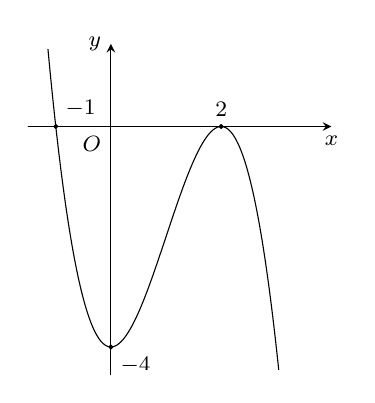
\begin{tikzpicture}[scale=0.7,>=stealth, font=\footnotesize, line join=round, line cap=round]
			\def\a{-1} \def\b{3} \def\c{0} \def\d{-4} % Hệ số
			\def\xmin{-1.5} \def\xmax{4}
			\def\ymin{-4.5} \def\ymax{1.5} 
			\draw[->] (\xmin,0)--(\xmax,0) node [below]{$x$};
			\draw[->] (0,\ymin)--(0,\ymax) node [left]{$y$};
			\node at (0,0) [below left]{$O$};
			\clip (\xmin+0.1,\ymin+0.1) rectangle (\xmax-0.5,\ymax-0.1);
			\draw[smooth,samples=300] plot(\x,{\a*(\x)^3+\b*(\x)^2+\c*(\x)+\d});
			\draw[fill=black](2,0)node[above]{$2$}circle(1pt)
			(-1,0)node[above right]{$-1$}circle(1pt)
			(0,-4)node[below right]{$-4$}circle(1pt)
			;
	\end{tikzpicture}}
	\loigiai{
		Từ đồ thị, ta thấy hàm số đồng biến trên khoảng $(0; 2)$.
	}
\end{ex}
\begin{ex}%[2D1N2-2]
	\immini{Cho hàm số $y=f(x)$ có đồ thị như hình vẽ. Toạ độ điểm cực đại của đồ thị hàm số đã cho là
		\choice[2]
		{$(-1;0)$}
		{$(0;1)$}
		{$(-1;1)$}
		{\True $(1;3)$}}
	{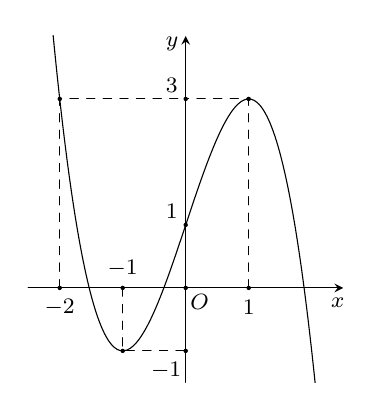
\begin{tikzpicture}[scale=0.8, font=\footnotesize, line join=round, line cap=round, >=stealth,declare function={f(\x)=-(\x)^3+3*(\x)+1;}]
			\def \xmin{-2.5}
			\def \xmax{2.5}
			\def \ymin{-1.5}
			\def \ymax{4}
			\draw[->] (\xmin,0)--(\xmax,0) node[shift=(-110:0.2)] {$x$};
			\draw[->] (0,\ymin)--(0,\ymax) node[shift=(-150:0.2)] {$y$};
			\clip (\xmin,\ymin) rectangle (\xmax,\ymax);
			\fill (0,0) circle(1pt) node[shift=(-45:0.25)]{$O$}
			(-2,0) circle(1pt) node[shift=(-90:0.25)]{$-2$}
			(-1,0) circle(1pt) node[shift=(90:0.25)]{$-1$}
			(1,0) circle(1pt) node[shift=(-90:0.25)]{$1$}
			(0,-1) circle(1pt) node[shift=(-135:0.35)]{$-1$}
			(0,1) circle(1pt) node[shift=(135:0.25)]{$1$}
			(0,3) circle(1pt) node[shift=(135:0.25)]{$3$}
			(-2,3) circle(1pt) (-1,-1) circle(1pt) (1,3) circle(1pt);
			\draw[dashed] (-2,0)|-(0,3) (-1,0)|-(0,-1) (1,0)|-(0,3);
			\draw[smooth,samples=100,domain=\xmin:\xmax] plot(\x, {f(\x)});
	\end{tikzpicture}}
	\loigiai{
		Dựa vào đồ thị hàm số đã cho, tọa độ điểm cực đại của đồ thị hàm số có tọa độ $(1;3)$.
	}
\end{ex}
\begin{ex}%[2D1N3-1]
	\immini{Cho hàm số $y=f(x)$ có đồ thị như hình vẽ. Gọi $M$, $m$ lần lượt là giá trị lớn nhất và giá trị nhỏ nhất của hàm số trên $[-2; 2]$. Phát biểu nào sau đây là đúng?
		\choice
		{$M+m=0$}
		{$M-m=2$}
		{\True $2M+m=5$}
		{$2M-m=5$}}
	{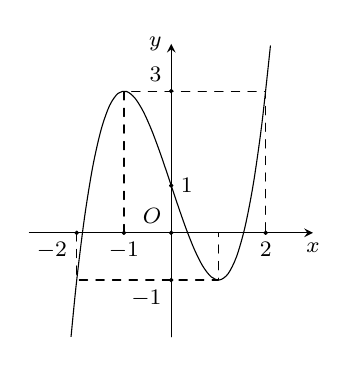
\begin{tikzpicture}[scale=.6, line join=round, line cap=round, >=stealth,
			declare function={
				f(\x)=(\x)^3-3*(\x)+1;
			}
			]
			\draw[->] (-3,0)--(0,0)node[above left]{\footnotesize $O$}--(3,0) node[below]{\footnotesize $x$};
			\draw[->] (0,-2.2)--(0,4) node[left]{\footnotesize $y$};
			\draw[dashed] (-1,0)--(-1,3)--(2,3)--(2,0);	
			\draw[dashed] (-2,0)--(-2,-1)--(1,-1)--(1,0);
			\begin{scope}
				\clip (-3,-2.2) rectangle (3,4);
				\draw[smooth] plot[domain=-2.2:2.1] ({\x},{f(\x)});
			\end{scope}
			\foreach \x in {-1,2}
			\draw[fill=black] (\x,0) node[below]{\footnotesize $\x$} circle(1pt);
			\foreach \y in {1}
			\draw[fill=black] (0,\y) node[right]{\footnotesize $\y$} circle(1pt);
			\foreach \y in {-1}
			\draw[fill=black] (0,\y) node[below left]{\footnotesize $\y$} circle(1pt);
			\foreach \y in {3}
			\draw[fill=black] (0,\y) node[above left]{\footnotesize $\y$} circle(1pt);
			\draw[fill=black] (-2,0) node[below left]{\footnotesize $-2$} circle(1pt);
			\draw[fill=black] (0,0) circle(1pt);
	\end{tikzpicture}}
	\loigiai{
		Dựa vào đồ thị hàm số ta được $M=3$, $m=-1$ nên $2M+m=3\cdot2-1=5$.
	}
\end{ex}
\begin{ex}%[2D1H3-1]
	Giá trị lớn nhất của hàm số $y=x^4-4x^2+9$ trên đoạn $[-2 ; 3]$ bằng
	\choice
	{$201$}
	{$2$}
	{$9$}
	{\True $54$}
	\loigiai{
		Hàm số đã cho liên tục trên đoạn $[-2;3]$.\\
		Ta có	$y'=4x^3-8x$; $y'=0 \Leftrightarrow \hoac{
			&x=0\\
			&x=\pm\sqrt{2}.}$\\
		Ta có $y(-2)=9$; $y(3)=54$; $y(0)=9$; $y\left(\pm\sqrt{2}\right)=5$.\\
		Vậy $\max\limits_{[-2 ; 3]} y=y(3)=54$.
	}
\end{ex}
\begin{ex}%[2D1N4-1]
	\immini{
		Cho hàm số $y=\dfrac{ax+b}{cx+d}$  ($c\ne 0$, $ad-bc\ne 0$) có đồ thị như hình vẽ bên. Tiệm cận đứng và tiệm cận ngang của đồ thị lần lượt là
		\choice
		{\True $x=-1$ và $y=2$}
		{$x=1$ và $y=2$}
		{$x=-1$ và $y=-2$}
		{$x=1$ và $y=-2$}
	}{
		\begin{tikzpicture}[scale=0.5, font=\footnotesize, line join=round, line cap=round, >=stealth]
			\def \f{(2*(\x)+3)/(1*(\x)+1)} %%Hàm số
			\def \xo{-1} %Tiệm cận đứng
			\def \yo{2} %Tiệm cận ngang
			\def \k{5} %Độ rộng của đồ thị
			\draw[->] (\xo-\k,0)--(\xo+\k,0) node[below left] {$x$};
			\draw[->] (0,\yo-\k)--(0,\yo+\k) node[below left] {$y$};
			\draw (0,0) node [below right] {$O$};
			%Vẽ các điểm trên trục Ox
			\foreach \x/\g in {-1/-90}
			\draw[thin] (\x,2pt)--(\x,-2pt) + (\g:5mm) node {\scriptsize $\x$};
			%Vẽ các điểm trên trục Oy
			\foreach \y/\g in {2/-60,3/180}
			\draw[thin] (2pt,\y)--(-2pt,\y) + (\g:5mm) node {\scriptsize $\y$};
			\begin{scope}
				\clip (\xo-\k,\yo-\k) rectangle (\xo+\k,\yo+\k);
				\draw[smooth,samples=200,domain=\xo-\k:\xo-0.1,smooth,variable=\x] plot (\x,{\f});
				\draw[smooth,samples=200,domain=\xo+0.1:\xo+\k,smooth,variable=\x] plot (\x,{\f});
				%Tiệm cận
				\draw[dashed,thin] 
				(\xo,\yo-\k)--(\xo,\yo+\k)  (\xo-\k,\yo)--(\xo+\k,\yo);
			\end{scope}
		\end{tikzpicture}
	}
	\loigiai{
		Nhìn vào đồ thị ta suy ra  tiệm cận đứng và tiệm cận ngang lần lượt là các đường thẳng $x=-1$; $y=2$.
	}
\end{ex}
\begin{ex}%[2D1N4-1]
	Trong các hàm số sau đây, hàm số nào có đồ thị nhận đường thẳng $x=1$ làm đường tiệm cận đứng?
	\choice
	{\True $y=\dfrac{2x-1}{x-1}$}
	{$y=\dfrac{x^2+2x-3}{2x-3}$}
	{$y=x-\sqrt{x^2+2}$}
	{$y=\dfrac{2}{x^2+x+1}$}
	\loigiai{
		Xét hàm số $y=\dfrac{2x-1}{x-1}$.\\
		Ta có $\lim\limits_{x \to 1^+}\, \dfrac{2x-1}{x-1}=+\infty$ và $\lim\limits_{x \to 1^-}\, \dfrac{2x-1}{x-1}=-\infty$.\\
		Do đó, hàm số $y=\dfrac{2x-1}{x-1}$ có đồ thị nhận đường thẳng $x=1$ làm đường tiệm cận đứng.
	}
\end{ex}
\begin{ex}%[2D1N4-1]
	Tiệm cận xiên của đồ thị hàm số $y = x - 1 + \dfrac{3}{x+1}$ đi qua điểm nào sau đây?
	\choice
	{ Điểm $M(0; 1)$ }
	{\True Điểm $N(0; -1)$ }
	{ Điểm $P(1; 1)$ }
	{ Điểm $Q(-1; 0)$ }
	\loigiai{
		Ta có $\lim\limits_{x \to \pm\infty} \left[ y - (x-1) \right] = \lim\limits_{x \to \pm\infty} \dfrac{3}{x+1} = 0$.\\
		Vậy tiệm cận xiên của đồ thị hàm số đã cho là đường thẳng $d\colon y = x - 1$.\\
		Dễ dàng ta thấy đường thẳng $d$ đi qua điểm $N(0; -1)$. 
	}
\end{ex}
\begin{ex}%[2D1H5-1]%[Đắc Vũ]
	\immini{
		Đường cong trong hình bên là đồ thị của hàm số
		\choice
		{$y=x^3+3x^2-2$}
		{\True $y=-x^3+3x^2-2$}
		{$y=x^3-3x^2-2$}
		{$y=-x^3+3x^2+2$}
	}{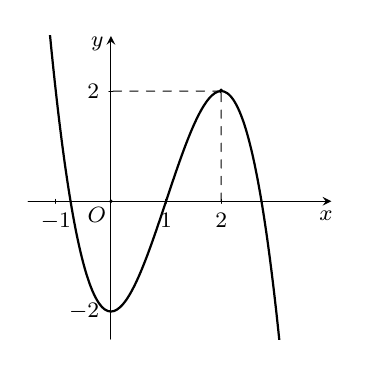
\begin{tikzpicture}[scale=0.7, font=\footnotesize, line join=round,
			line cap=round, >=stealth]
			\def \xmin{-1.5}
			\def \xmax{4}
			\def \ymin{-2.5}
			\def \ymax{3}
			\draw[->] (\xmin,0)--(\xmax,0) node[shift=(-110:0.2)] {$x$};
			\draw[->] (0,\ymin)--(0,\ymax) node[shift=(-150:0.2)] {$y$};
			\fill (0,0) circle(1pt) node[shift=(-135:0.25)]{$O$};
			\clip (\xmin,\ymin) rectangle (\xmax,\ymax);
			\draw[smooth,samples=100,domain=\xmin:\xmax,thick] plot(\x,{-(\x)^3+3*(\x)^2-2});
			\foreach  \x/\nx in {1/1,2/2,-1/-1} 
			\draw (\x,1pt)--(\x,-1pt)  node[below] {$\nx$};
			\foreach  \y/\ny in {2/2,-2/-2} 
			\draw (1pt,\y)--(-1pt,\y)node[left] {$\ny$};
			\draw[dashed] (2,0)--(2,2) circle(1pt)--(0,2);
	\end{tikzpicture}}
	\loigiai{Giả sử hàm số cần tìm có dạng là $y=ax^3+bx^2+cx+d \ (a\ne 0)$.\\
		Đồ thị hàm số đi qua các điểm $(0;-2)$, $(1;0)$, $(2;2)$ và có điểm cực trị $(0;-2)$ nên ta có 
		\[\heva{&d=-2\\&a+b+c+d=1\\&8a+4b+2c+d=2\\&c=0} \Leftrightarrow \heva{&a=-1\\&b=3\\&c=0\\&d=-2.}\]
		Suy ra hàm số cần tìm là $y=-x^3+3x^2-2$.}
\end{ex}
\begin{ex}%[2D1H5-1]
	\immini
	{
		Cho hàm số $y=\dfrac{ax+3}{bx+c}$ có đồ thị là đường cong trong hình vẽ.
		Tính giá trị $M=a+b+c$.
		\choice
		{$0$}
		{\True $4$}
		{$3$}
		{$-1$}
	}
	{
		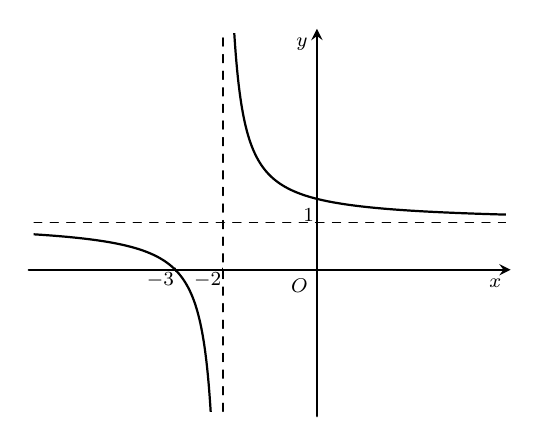
\begin{tikzpicture}[line join=round, line cap=round,>=stealth,thick,font=\footnotesize,scale=0.6]
			\tikzset{every node/.style={scale=0.9}}
			\draw[->] (-6.1,0)--(4.1,0) node[below left] {$x$};
			\draw[->] (0,-3.1)--(0,5.1) node[below left] {$y$};
			\draw (0,0) node [below left] {$O$};
			\foreach \x/\nx in {-3/-3,-2/-2}
			\draw[thin] (\x,1pt)--(\x,-1pt) node [below left=-3pt] {$\nx$};
			\foreach \y/\ny in {1/1}
			\draw[thin] (1pt,\y)--(-1pt,\y) node [above left=-3pt] {$\ny$};
			\draw[dashed,thin] (-1.99,-3)--(-1.99,5);
			\begin{scope}
				\clip (-6,-3) rectangle (4,5);
				\draw[samples=200,domain=-6:-2.01,smooth,variable=\x] plot (\x,{(1*(\x)+3)/(1*(\x)+2)});
				\draw[samples=200,domain=-1.99:4,smooth,variable=\x] plot (\x,{(1*(\x)+3)/(1*(\x)+2)});
				\draw[dashed,thin] (-6,1/1)--(4,1/1);
			\end{scope}
		\end{tikzpicture}
	}
	\loigiai{
		Đồ thị đi qua điểm $(-3;0)$ nên $0=\dfrac{-3\cdot a+3}{-3\cdot b+c} \Rightarrow -3\cdot a+3=0 \Leftrightarrow a=1$.\\
		Đồ thị hàm số có tiệm cận ngang $y=1$ nên $\dfrac{a}{b}=1 \Leftrightarrow b=a=1$.\\
		Đồ thị hàm số có tiệm cận đứng $x=-2$ nên $-\dfrac{c}{b}=-2 \Leftrightarrow c=2b=2$.\\
		Vậy $M=a+b+c=1+1+2=4$.
	}
\end{ex}
\begin{ex}%[2D1H5-7]
	Cho hàm số $f(x) = \dfrac{mx^2 + nx + p}{qx + r}$ có bảng biến thiên như sau
	\begin{center}
		
\begin{tikzpicture}
			\tkzTabInit[nocadre=false,lgt=1.2,espcl=2,deltacl=0.5]{$x$/.6 ,$f'(x)$/.6,$f(x)$/2}
			{$-\infty$ , $x_1$ , $-1$ , $x_2$ , $+\infty$}
			\tkzTabLine{ , + , $0$ , - , d , - , $0$ , + , }
			\tkzTabVar{-/$-\infty$ , +/$-5$ , -D+/$-\infty$/$+\infty$ , -/$3$ , +/$+\infty$}
		\end{tikzpicture}
	\end{center}
	Gọi $I$ là tâm đối xứng của đồ thị hàm số $y = f(x)$. Tìm tọa độ $I$.
	\choice
	{$I(-2;1)$}
	{$I(-1;1)$}
	{$I(-1;0)$}
	{\True $I(-1;-1)$}
	\loigiai{
		Ta có $I$ là tâm đối xứng của đồ thị hàm số $y = f(x)$, do đó hai điểm cực trị đối xứng qua $I$.\\
		Suy ra $x_I = -1$; $y_I = \dfrac{-5 + 3}{2} = -1$.\\
		Vậy $I(-1;-1)$.
	}
\end{ex}
\Closesolutionfile{ans}
%\begin{center}
%	\textbf{ĐÁP ÁN}
%	\inputansbox{10}{ans/ans}	
%\end{center}
\begin{center}
	\textbf{PHẦN 2 - CÂU TRẮC NGHIỆM ĐÚNG SAI}
\end{center}
\setcounter{ex}{0}
\Opensolutionfile{ans}[ans/answer-DS-ONTAPCHUONG-DE1]
\begin{ex}%[2D1N2-2]
	\immini{Cho hàm số $y = f(x)$ có đồ thị như hình vẽ.
		\choiceTF
		{\True Hàm số đạt cực đại tại $x = 1$}
		{Hàm số nghịch biến trên khoảng $(-1;1)$}
		{Tổng giá trị cực đại và cực tiểu của hàm số bằng $-4$}
		{Hàm số đồng biến trên khoảng $(-3;1)$}
	}
	{
		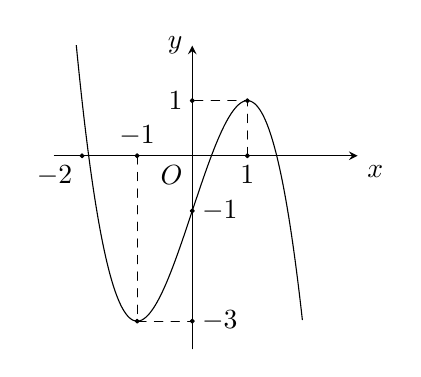
\begin{tikzpicture}[>=stealth, line cap= round, line join=round, scale=0.7]
			\def\xmin{-2.5};\def\xmax{3};\def\ymin{-3.5};\def\ymax{2};
			\draw[->] (\xmin,0)--(\xmax,0) node[below right] {$x$};
			\draw[->] (0,\ymin)--(0,\ymax) node[left] {$y$};
			\draw (0,0) node [below left] {$O$};
			\begin{scope}
				\clip (\xmin,\ymin) rectangle (\xmax,\ymax);
				\draw[samples=200,domain=-2.5:2,smooth,variable=\x] plot (\x,{-(\x)^3+3*(\x)-1});
			\end{scope}
			\draw[fill=black] (1,0)circle(1pt)node[below]{$1$}
			(-1,0)circle(1pt)node[above]{$-1$}
			(-2,0)circle(1pt)node[below left]{$-2$}
			(0,1)circle(1pt)node[left]{$1$}
			(0,-1)circle(1pt)node[right]{$-1$}
			(0,-3)circle(1pt)node[right]{$-3$}
			(-1,-3)circle(1pt)
			(1,1)circle(1pt)
			;
			\draw[dashed] (-1,0)|-(0,-3) (1,0)|-(0,1)
			;
		\end{tikzpicture}
		
	}
	\loigiai{
		\begin{itemchoice}
			\itemch 
			Dựa vào đồ thị, hàm số đạt cực đại tại $x = 1$.
			\itemch 
			Hàm số đồng biến trên $(-1;1)$.
			\itemch 
			Hàm số có giá trị cực đại $y_{\text{CĐ}}=1$ và $y_{\text{CT}}=-3$. Do đó $y_{\text{CĐ}}+y_{\text{CT}}=-2$.
			\itemch 
			Hàm số nghịch biến trên $(-3;-1)$ nên không thể đồng biến trên $(-3;1)$.
		\end{itemchoice}
	}
\end{ex}
\begin{ex}%[2D1H4-3]
	Cho hàm số $(C_1)\colon y = f(x) = \dfrac{3x-1}{x-2}$; $(C_2)\colon y = g(x) = x-1 - \dfrac{2}{2x-1}$.
	\choiceTF
	{Hàm số $y = f(x)$ luôn nghịch biến trên $\mathbb{R}$}
	{\True $\max\limits_{[1;2]} g(x) = \dfrac{1}{3}$, $\min\limits_{[1;2]} g(x) = -2$}
	{Đồ thị hàm số $y = f(x)$ có tiệm cận đứng và tiệm cận ngang tạo với $2$ trục tọa độ một đa giác có chu vi bằng $6$}
	{\True Hai đường tiệm cận của đồ thị hàm số $y = f(x)$ cùng với đường tiệm cận xiên của đồ thị hàm số $y = g(x)$ tạo thành tam giác có diện tích bằng $2$}
	\loigiai{
		\begin{itemchoice}
			\itemch 
			Tập xác định của hàm số $y=f(x)$ là $\mathscr{D}=\mathbb{R}\setminus\{2\}$ nên hàm số $y=f(x)$ không nghịch biến trên $\mathbb{R}$.
			\itemch 
			Ta có $g'(x) = 1 + \dfrac{4}{(2x-1)^2} > 0$, $\forall x \ne \dfrac{1}{2}$.\\
			Mặt khác $g(1) = -2$, $g(2) = \dfrac{1}{3}$.\\
			Do đó $\max\limits_{[1;2]} g(x) = \dfrac{1}{3}$, $\min\limits_{[1;2]} g(x) = -2$.
			\itemch 
			Vì $\lim\limits_{x \to \pm\infty} f(x) = \lim\limits_{x \to \pm\infty} \dfrac{3x-1}{x-2} = \lim\limits_{x \to \pm\infty} \dfrac{3-\dfrac{1}{x}}{1-\dfrac{2}{x}} = 3$.\\
			Nên đồ thị hàm số $y=f(x)$ có một tiệm cận ngang là $y=3$.\\
			Vì $\lim\limits_{x \to 2^+} f(x) = \lim\limits_{x \to 2^+} \dfrac{3x-1}{x-2} = +\infty$.\\
			Nên đồ thị hàm số $y=f(x)$ có một tiệm cận đứng là $x=2$.\\
			Do đó hàm số $y = f(x)$ có tiệm cận đứng và tiệm cận ngang tạo với $2$ trục tọa độ một hình chữ nhật có chiều dài bằng $3$, chiều rộng bằng $2$ nên có chu vi bằng $2\cdot(3+2)=12$.
			\itemch 
			Ta có $\lim\limits_{x \to +\infty} \left[g(x) - (x-1)\right] =\lim\limits_{x \to +\infty} \left[- \dfrac{2}{2x-1}\right] =0$.\\
			Suy ra tiệm cận xiên của đồ thị hàm số $y=g(x)$ là đường thẳng $d\colon y=x-1$.\\
			Giao điểm hai đường tiệm cận của đồ thị hàm số $y=f(x)$ là $A(2;3)$.\\
			Giao điểm đường tiệm cận đứng của đồ thị hàm số $y=f(x)$ và đường tiệm cận xiên của đồ thị hàm số $y=g(x)$ là $B(2;1)$.\\
			Giao điểm đường tiệm cận ngang của đồ thị hàm số $y=f(x)$ và đường tiệm cận xiên của đồ thị hàm số $y=g(x)$ là $C(4;3)$.\\
			Mặt khác hai đường tiệm cận của đồ thị hàm số $y=f(x)$ vuông góc với nhau nên tam giác $ABC$ vuông tại $A$.\\
			Ta có $AB=\left|1-3\right|=2$, $AC=\left|4-2\right|=2$.\\
			Suy ra $S_{\triangle ABC} = \dfrac{1}{2}\cdot AB\cdot AC = 2$.
		\end{itemchoice}
	}
\end{ex}
\Closesolutionfile{ans}
%\inputansbox[2]{2}{ans/answer.tex}



\begin{center}
	\textbf{PHẦN 3 - CÂU TRẮC NGHIỆM TRẢ LỜI NGẮN}
\end{center}
\setcounter{ex}{0}
\Opensolutionfile{ans}[ans-KQ-ONTAPCHUONG-DE1]
\begin{ex}%[2D1H2-1]
	Đồ thị hàm số $y=f(x)=x^3-3x^2-9x+1$ có hai điểm cực trị là $A$, $B$. Tìm khoảng cách giữa hai điểm $A$ và $B$. (Kết quả làm tròn đến hàng phần mười)
	\shortans{32,2}
	\loigiai{
		Ta có $y'=3x^2-6x-9=0 \Leftrightarrow \hoac{&x=-1\\&x=3.}$\\
		Suy ra đồ thị hàm số có 2 điểm cực trị $A\left(-1;6\right)$ và $B\left(3;-26\right)$.\\
		Vậy khoảng cách giữa hai điểm $A$ và $B$ là $AB=\sqrt{1\,040}\approx 32{,}2$.
	}
\end{ex}
\begin{ex}%[2D1N4-1]
	Đồ thị hàm số $y = \dfrac{x^2-2x+5}{x^2-1}$ có bao nhiêu đường tiệm cận?
	\shortans[oly]{3}
	\loigiai{
		Tập xác định của hàm số là $\mathscr{D}=\mathbb{R} \setminus \{-1;1\}$.\\
		Ta có 
		\begin{itemize}
			\item $\lim\limits_{x\to \pm \infty}y=\lim\limits_{x\to \pm \infty} \left(\dfrac{x^2-2x+5}{x^2-1}\right)=\lim\limits_{x\to \pm \infty} \left(\dfrac{1-\dfrac{2}{x}+\dfrac{5}{x^2}}{1-\dfrac{1}{x^2}}\right)=1$.\\
			Do đó $y=1$ là tiệm cận ngang của đồ thị hàm số.
			\item $\lim\limits_{x\to 1^{+}}y=\lim\limits_{x\to 1^{+}}\left(\dfrac{x^2-2x+5}{x^2-1}\right)=+\infty$.\\
			Do đó $x=1$ là tiệm cận đứng của đồ thị hàm số.
			\item $\lim\limits_{x\to -1^{+}}y=\lim\limits_{x\to -1^{+}}\left(\dfrac{x^2-2x+5}{x^2-1}\right)=-\infty$.\\
			Do đó $x=-1$ là tiệm cận đứng của đồ thị hàm số.
		\end{itemize}
		Vậy đồ thị hàm số có ba đường tiệm cận.
	}
\end{ex}
\begin{ex}%[2D1V3-6]
	Công ty sữa làm các lon đựng sữa hình trụ có thể tích $800$ cm$^3$ (lon sữa có nắp và bỏ qua việc gấp mí). Để chi phí vật liệu (thiếc) làm hộp sữa nhỏ nhất, cần thiết kế hộp sữa có bán kính bao nhiêu cm (\textit{chính xác đến hàng phần trăm})?
	\shortans[oly]{5,03}
	\loigiai{
		Gọi $R\ (R > 0)$ là bán kính của hình trụ, $h$ là chiều cao của hình trụ.\\
		Thể tích của lon sữa là $V = \pi R^2 h \Rightarrow h = \dfrac{V}{\pi R^2}$.\\
		Diện tích toàn phần của lon sữa $S_{tp} = 2\pi R^2 + 2\pi Rl$, vì $l = h = \dfrac{V}{\pi R^2}$ nên
		\[
		S_{tp} = 2\pi R^2 + 2\pi Rl = 2\pi R^2 + 2\pi R\cdot \dfrac{800}{\pi R^2} = 2\pi R^2 + \dfrac{1\,600}{R}.
		\]
		Chi phí vật liệu làm hộp sữa nhỏ nhất khi $S_{tp}$ nhỏ nhất.\\
		Xét hàm số $f(x)=2\pi x^2+\dfrac{1\,600}{x}$ với $x>0$.\\
		Ta có $f'(x)=4\pi x-\dfrac{1\,600}{x^2}=0 \Leftrightarrow x=\sqrt[3]{\dfrac{400}{\pi}}$.\\
		Bảng biến thiên
		\begin{center}
			
\begin{tikzpicture}
				\tkzTabInit[lgt=1.2, espcl=3]
				{$x$ /1, $f'(x)$ /1, $f(x)$ /2} 
				{$0$,$\sqrt[3]{\dfrac{400}{\pi}}$, $+\infty$}
				\tkzTabLine{,+,0,-,}
				\tkzTabVar{-/, +/$477$ ,-/}
			\end{tikzpicture}
		\end{center}
		Vậy để chi phí vật liệu làm hộp sữa nhỏ nhất, cần thiết kế hộp sữa có bán kính khoảng $5{,}03$ cm.
	}
\end{ex}
\begin{ex}%[2D1V3-6]
	Người ta muốn lắp một ống dẫn dầu từ nhà máy lọc dầu ở vị trí $A$ đến kho chứa dầu đặt ở vị trí $B$ qua một con sông rộng $2$ km, dài $6$ km. Chi phí lắp đặt đường ống dẫn dầu trên mặt đất để nối từ nhà máy lọc dầu đến trạm trung chuyển tại vị trí $P$ là $4$ tỷ VNĐ/$1$ km và chi phí lắp đặt đường ống dẫn dầu dưới dòng sông để nối từ $P$ đến kho chứa dầu tại vị trí $B$ là $8$ tỷ VNĐ/$1$ km (như hình vẽ).
	\begin{center}
		\begin{tikzpicture}[scale=1, font=\footnotesize, line join=round, line cap=round, >=stealth]
			\path 
			(0,0) coordinate (A)
			(0,-2) coordinate (H)
			(3,0) coordinate (P)
			(4,-2) coordinate (B)
			($(A)!(B)!(P)$) coordinate (K)
			;
			
			\draw ($(A)+(180:0.5)$)--($(P)+(0:1.5)$);
			\draw ($(H)+(180:0.5)$)--($(B)+(0:0.5)$);
			\draw[<->] ($(A)+(180:0.5)$)--node[left]{$2\text{ km}$}($(H)+(180:0.5)$);
			\draw[<->] ($(H)+(-90:1)$) --node[below]{$6\text{ km}$}($(B)+(-90:1)$);
			\draw (A)--(H) (B)--(P) (B)--(K);
			\foreach \p/\r in {A/90,B/-90,H/-90,P/90}
			\fill (\p) circle (1pt) node[shift={(\r:3mm)}]{$\p$};
		\end{tikzpicture}
	\end{center}
	Hỏi để chi phí lắp đặt ít nhất, cần đặt vị trí $P$ cách nhà máy lọc dầu là bao nhiêu kilômét? (làm tròn kết quả đến hàng phần trăm).
	\shortans{4,85}
	\loigiai{
		Đặt $AP=x$ (km) ($0\le x\le 6$).
		\begin{center}
			\begin{tikzpicture}[scale=1, font=\footnotesize, line join=round, line cap=round, >=stealth]
				\path 
				(0,0) coordinate (A)
				(0,-2) coordinate (H)
				(3,0) coordinate (P)
				(4,-2) coordinate (B)
				($(A)!(B)!(P)$) coordinate (K)
				;
				
				\draw ($(A)+(180:0.5)$)--($(P)+(0:1.5)$);
				\draw ($(H)+(180:0.5)$)--($(B)+(0:0.5)$);
				\draw[<->] ($(A)+(180:0.5)$)--node[left]{$2\text{ km}$}($(H)+(180:0.5)$);
				\draw[<->] ($(H)+(-90:1)$) --node[below]{$6\text{ km}$}($(B)+(-90:1)$);
				\draw (A)--(H) (B)--(P) (B)--(K);
				\foreach \p/\r in {A/90,B/-90,H/-90,P/90,K/90}
				\fill (\p) circle (1pt) node[shift={(\r:3mm)}]{$\p$};
			\end{tikzpicture}
		\end{center}
		Khi đó, chiều dài quãng đường $PK=6-x$.\\
		Tổng chi phí lắp đặt đường ống dẫn dầu là $T(x)=4x+8\sqrt{\left(6-x\right)^2+2^2}$ (tỷ VNĐ).\\
		Ta có $T'(x)=4+8\dfrac{x-6}{\sqrt{x^2-12x+40}}$.\\
		Xét 
		\begin{eqnarray*}
			& &T'(x)=0\Leftrightarrow 4\sqrt{x^2-12x+40}+8x-48=0\\
			&\Leftrightarrow& \sqrt{x^2-12x+40}=12-2x\,\left(\text{Điều kiện }0<x\le 6\right)\\
			&\Leftrightarrow& 3x^2-36x+104=0\Leftrightarrow x=\dfrac{18\pm 2\sqrt{3}}{3}.
		\end{eqnarray*}
		Kết hợp điều kiện ta thấy $x=\dfrac{18-2\sqrt{3}}{3}\approx 4{,}85$ là nghiệm của phương trình.\\
		Ta có bảng biến thiên
		\begin{center}
			
\begin{tikzpicture}
				\tkzTabInit[nocadre=false,lgt=1.2,espcl=2.5,deltacl=0.6]
				{$x$ /0.6,$T'(x)$ /0.6,$T(x)$ /2}
				{$0$,$4{,}85$,$6$}
				\tkzTabLine{,-,0,+,}
				\tkzTabVar{+/,-/,+/}
			\end{tikzpicture}
		\end{center}
		Từ bảng biến thiên ta suy ra chi phí thấp nhất khi $x=4{,}85$.}
\end{ex}
\Closesolutionfile{ans}



\begin{center}
	\textbf{PHẦN 4 - TỰ LUẬN}
\end{center}
\setcounter{ex}{0}
\begin{ex}%[2D1H2-1]
	Tìm cực trị của hàm số $y=x^3-3 x^2+1$.
	\loigiai{
		Tập xác định của hàm số là $\mathscr{D}=\mathbb{R}$. \\
		Ta có  $y'=3 x^{2}-6 x$.\\
		Khi đó		$y'=0 \Leftrightarrow \hoac{&x=0 \\ &x=2.}$\\
		Ta có bảng biến thiên
		\begin{center}
			
\begin{tikzpicture}
				\tkzTabInit[lgt=1.2, espcl=3]
				{$x$ /1, $y'$ /1, $y$ /2} 
				{$-\infty$,$0$,$2$, $+\infty$}
				\tkzTabLine{,+,0,-,0,+,}
				\tkzTabVar{-/ $-\infty$, +/$1$ ,-/$-3$, +/ $+\infty$}
			\end{tikzpicture}
		\end{center}
		Từ bảng biến thiên, ta có
		\begin{itemize}
			\item Hàm số đạt cực đại tại $x=0$ và $y_{\text{CĐ}}=y(0)=1$.
			\item Hàm số đạt cực tiểu tại $x=-2$ và $y_{\text{CT}}=y(2)=-3$.
		\end{itemize}
	}
\end{ex}
\begin{ex}%[2D1V3-6]
	Nhà máy $A$ chuyên sản xuất một loại sản phẩm cung cấp cho nhà máy $B$. Hai nhà máy thoả thuận rằng, hàng tháng nhà máy $A$ cung cấp cho nhà máy $B$ số lượng sản phẩm theo đơn đặt hàng của $B$ (tối đa $100$ tấn sản phẩm). Nếu số lượng đặt hàng là $x$ tấn sản phẩm thì giá bán cho mỗi tấn sản phẩm là $P(x)=45-0{,}001 x^2$ (triệu đồng). Chi phí để $A$ sản xuất $x$ tấn sản phẩm trong một tháng gồm $100$ triệu đồng chi phí cố định và $30$ triệu đồng cho mỗi tấn sản phẩm. Nhà máy $A$ cần bán cho nhà máy $B$ bao nhiêu tấn sản phẩm mỗi tháng để lợi nhuận thu được lớn nhất? (làm tròn kết quả đến hàng phần mười).
	\loigiai{
		Số tiền (triệu đồng) mà nhà máy $A$ thu được từ việc bán $x$ tấn sản phẩm $(0 \leq x \leq 100)$ cho nhà máy $B$ là 
		\[
		R(x)=x \cdot P(x)=x\left(45 - 0{,}001 x^2\right) = 45x - 0{,}001 x^3.
		\]
		
		Chi phí (triệu đồng) để $A$ sản xuất $x$ tấn sản phẩm trong một tháng là
		\[
		C(x) = 100 + 30x.
		\]
		
		Lợi nhuận (triệu đồng) mà nhà máy $A$ thu được là
		\[
		L(x) = R(x) - C(x) = x\left(45 - 0{,}001 x^2\right) - (100 + 30x) = -0{,}001 x^3 + 15x - 100.
		\]
		
		Xét hàm số
		\[
		L(x) = -0{,}001 x^3 + 15x - 100  \text{ với } 0 \leq x \leq 100.
		\]
		
		Ta có
		\[
		L'(x) = -0{,}003 x^2 + 15 = 0 
		\Leftrightarrow x^2 = 5\,000 
		\Leftrightarrow x = 50 \sqrt{2}.
		\]
		Khi đó, ta có
		\[
		L(0) = -100; \
		L(50 \sqrt{2}) = 500 \sqrt{2} - 100 \approx 607;  \
		L(100) = 400.
		\]
		Vậy nhà máy $A$ thu được lợi nhuận lớn nhất là $607$ triệu đồng khi bán $50 \sqrt{2} \approx 70{,}7$ tấn sản phẩm cho nhà máy $B$ mỗi tháng.
		
	}
\end{ex}
\begin{ex}%[2D1C5-8]
	Một hòn đảo nằm trong một hồ nước. Biết rằng đường cong tạo nên hòn đảo được mô hình hoá vào hệ trục toạ độ $Oxy$ là một phần của đồ thị hàm số bậc ba $y=f(x)$ (tham khảo hình vẽ).
	\begin{center}
		\begin{tikzpicture}[font=\footnotesize ,line cap=round,line join=round,scale=.8,>=stealth]
			\draw[->] (-1,0)--(5,0) node[below right] {$x$};
			\draw[->] (0,-1)--(0,5) node[left] {$y$};
			\draw (0,0) node [below left] {$O$};
			\begin{scope}
				\clip (-1,-1) rectangle (5, 5);
				\draw[domain= 0:3.2,line width=.7 ,smooth,variable=\x] plot (\x,{-(\x)^3+3*(\x)^2});
				\draw[domain= 2.5:4.5,line width=.7 ,smooth,variable=\x] plot (\x,{16-4*(\x)});
			\end{scope}
			\draw (2.8,5)node[right]{$y=16-4x$};
			\draw(1.7,1)node[above]{Hòn đảo};
			\draw(4.6,1.5)node[above]{Mặt đường};
			\draw(1.2,3.75)node[above]{$f(x)$};
		\end{tikzpicture}
	\end{center}
	Vị trí điểm cực đại là $(2;4)$ với đơn vị của hệ trục là $100$ (m) và vị trí điểm cực tiểu là gốc toạ độ $O$. Mặt đường chạy trên một đường thẳng có phương trình $y=16-4x$. Người ta muốn làm một cây cầu có dạng một đoạn thẳng nối từ hòn đảo ra mặt đường. Độ dài ngắn nhất của cây cầu bằng bao nhiêu mét (làm tròn kết quả đến hàng phần mười)?
	\loigiai
	{
		Gọi hàm bậc ba $y=f(x)=ax^3+bx^2+cx+d\Rightarrow f'(x)=3ax^2+2bx+c$ với $a \ne 0$.\\
		Hàm số đi qua gốc toạ độ $\Rightarrow d=0\Rightarrow y=ax^3+bx^2+cx$.\\
		Hàm số có hai điểm cực trị $x=0$, $x=2\Rightarrow\heva{ & f'(0)=0 \\ &f'(2)=0 }\Rightarrow\heva{ & c=0 \\ &12a+4b+c=0 }\Rightarrow 3a+b=0$.\\
		Hàm số đi qua điểm $(2;4)\Rightarrow 8a+4b=4\Rightarrow 2a+b=1$.\\
		Từ đó suy ra $\heva{& a=-1 \\ &b=3}$. Suy ra $y=f(x)=-x^3+3x^2$.\\
		Gọi $M\left (x_0;y_0\right )$, $x_0>0$ là điểm nằm trên hòn đảo và nối với mặt đường, $d$ là tiếp tuyến của đồ thị hàm số tại $M$ và song song với mặt đường.\\
		Khi đó ta có 
		\[f'(x_0)=-4 \Leftrightarrow -3 x_0^2+6x_0=-4 \Leftrightarrow \hoac{x=1+\dfrac{\sqrt{21}}{3} \text{ (Nhận)}\\x=1-\dfrac{\sqrt{21}}{3} \text{ (Loại)}.}\]
		Độ dài cây cầu ngắn nhất bằng khoảng cách từ điểm $M \left(1+\dfrac{\sqrt{21}}{3}; 2+\dfrac{2\sqrt{21}}{9}\right)$ đến đường thẳng $\Delta\colon 4x+y-16=0$.\\
		Ta có
		\[\mathrm{d}(M,\Delta )=\dfrac{\left |4\cdot \left (1+\dfrac{\sqrt{21}}{3}\right )+2+\dfrac{2\sqrt{21}}{9}-16\right |}{\sqrt{4^2+1^2}}\cdot 100 \approx 69{,}6 \text{ m}.\]
	}
\end{ex}